% VUT FIT MITAI
% MSZ 2021/2022
% Author: Vladimir Dusek
% Login: xdusek27

%%%%%%%%%%%%%%%%%%%%%%%%%%%%%%%%%%%%%%%%%%%%%%%%%%%%%%%%%%%%%%%%%%%%%%%%%%%%%%%%

% Path to figures
\graphicspath{{sui/neuronove_site_a_jejich_trenovani/figures}}

%%%%%%%%%%%%%%%%%%%%%%%%%%%%%%%%%%%%%%%%%%%%%%%%%%%%%%%%%%%%%%%%%%%%%%%%%%%%%%%%

\chapter{SUI~--~Neuronové sítě a jejich trénování (metoda gradientního sestupu, účelová (loss) funkce, výpočetní graf, aktivační funkce, zápis pomocí maticového násobení, ...).}

%%%%%%%%%%%%%%%%%%%%%%%%%%%%%%%%%%%%%%%%%%%%%%%%%%%%%%%%%%%%%%%%%%%%%%%%%%%%%%%%

\section{Zdroje}

\begin{compactitem}
    \item \path{09-neural_networks.pdf}
    \item \path{SUI_2019-11-25.mp4}
    \item \path{SUI_2019-12-02.mp4}
\end{compactitem}

%%%%%%%%%%%%%%%%%%%%%%%%%%%%%%%%%%%%%%%%%%%%%%%%%%%%%%%%%%%%%%%%%%%%%%%%%%%%%%%%

\section{Neuronové sítě}

\begin{compactitem}
    \item Neuronové sítě jsou jedním z výpočetních modelů používaných v umělé inteligenci, resp. strojovém učení.

    \item Na nejvyšší abstrakci lze na neuronovou síť pohlížet jako na funkci, která dostane na vstup vektor (matici) reálných čísel a vrátí jiný vektor reálných čísel.
\end{compactitem}

\begin{figure}[H]
    \centering
    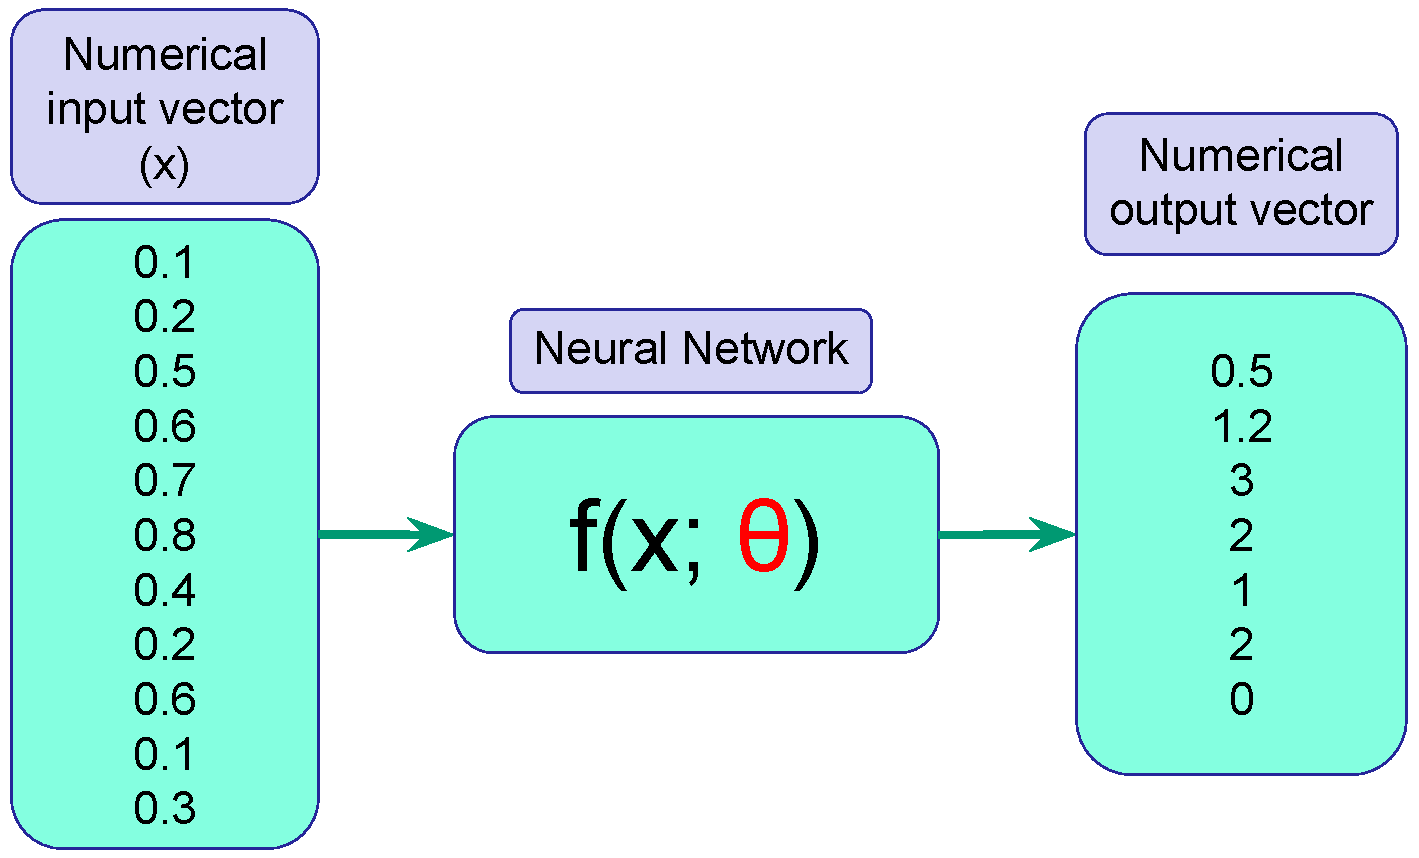
\includegraphics[width=0.65\linewidth]{neural_network_high_level.pdf}
    \caption{Neuronová síť jako funkce, $x$ je vektor vstupů, $\theta$ jsou parametry, které je třeba se naučit.}
\end{figure}

\subsection{Perceptron}

\begin{compactitem}
    \item Základní jednotka neuronové sítě se nazývána jako perceptron (také neuron).

    \item Vstup perceptronu je získáván z~výstupu jiných neuronů, či externího zdroje, pokud se jedná o perceptron ve vstupní vrstvě.

    \item Každému vstupu je přiřazen váhový koeficient, který určuje jeho relativní důležitost v~porovnání s~ostatními.

    \item Celkový výstup je vypočítán pomocí váženého součtu všech vstupů, aplikací aktivační funkce a přičtení zarovnávací hodnoty (\textit{bias}).

    \begin{equation}
        y=f(b + \sum_{i = 1}^{n} w_i x_i)
    \end{equation}
\end{compactitem}

\begin{figure}[H]
    \centering
    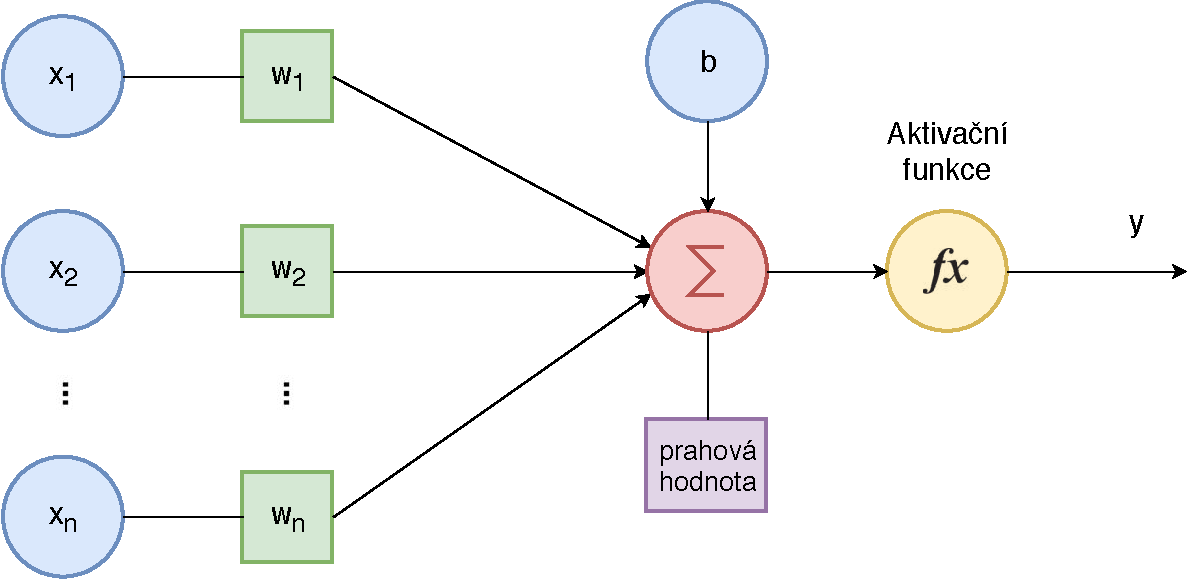
\includegraphics[width=0.7\linewidth]{perceptron.pdf}
    \caption{Perceptron.}
\end{figure}

\subsection{Vícevrstvé neuronové sítě}

\begin{compactitem}
    \item Použití pouze jednoho perceptronu není příliš efektivní, v praxi se setkáváme s~vícevrstvými neuronovými sítěmi (\textit{multi layer perceptron}).

    \item Jsou tvořeny opakováním perceptronu, které jsou na sebe napojeny ve vrstvách (počet vrstev a způsob propojení určuje architekturu sítě).

    \item Počet vstupních neuronů je dán počtem vstupů matematického modelu.

    \item Počet neuronů ve skryté vrstvě je volen s~ohledem na složitost úlohy. Čím složitější úloha, tím více neuronů je potřeba pro naučení se potřebných příznaků a pochopení struktury vzoru.

    \item Počet výstupních neuronů obvykle odpovídá počtu klasifikačních tříd (v případě klasifikační úlohy).

    \item Pokud má neuronová síť více skrytých vrstev, pak o ní hovoříme jako o~hluboké neuronové síti (\textit{deep neural network}).

    \item Jednotlivé skryté vrstvy mohou mít různé formy specializace (konvoluční, pooling, dropout, rekurentní, \dots)
\end{compactitem}

\begin{figure}[H]
    \centering
    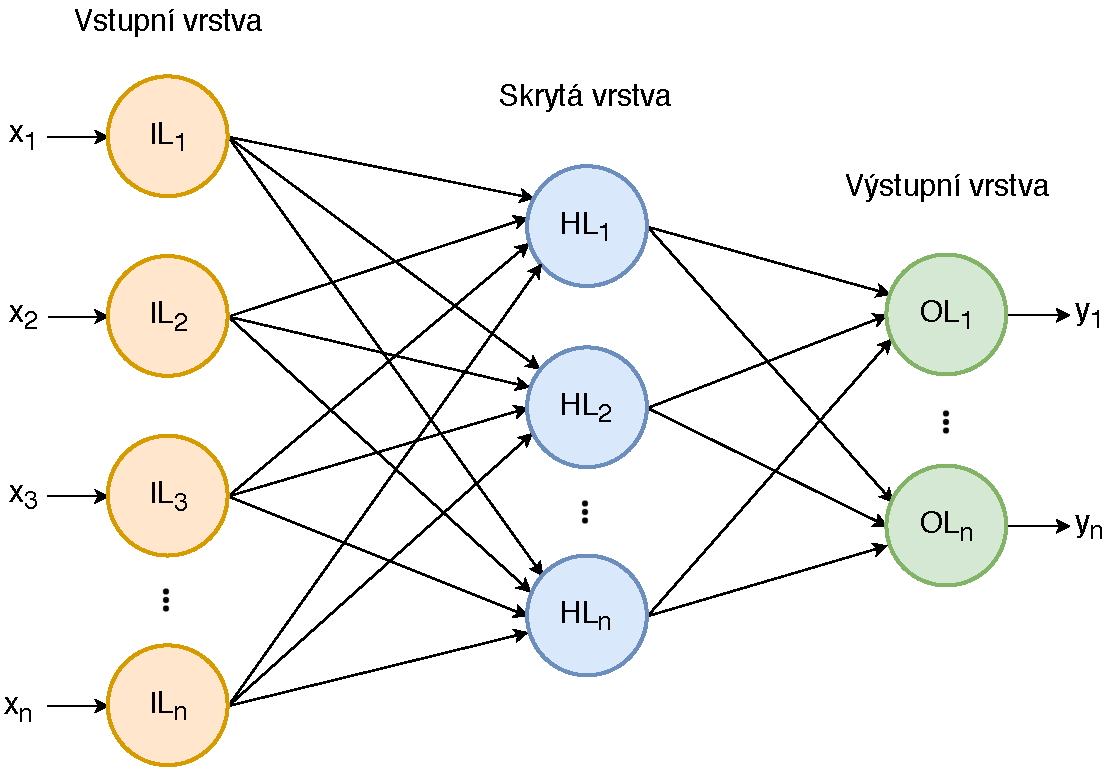
\includegraphics[width=0.7\linewidth]{multi_layer.pdf}
    \caption{Vícevrstvé neuronové sítě.}
\end{figure}

\subsection{Aktivační funkce}

\begin{compactitem}
    \item Aktivační funkce (také přenosová) slouží pro výpočet výstupní hodnoty neuronu v~závislosti na jeho vektoru vstupních hodnot.

    \item Proč jsou aktivační funkce potřeba:\begin{compactitem}

        \item Přidávají do výpočtu nelinearitu -- bez nich, by bylo možné libovolně velkou neuronovou síť vyjádřit jako jednu lineární fuknci!

        \item Bez aktivačních funkcí by výstup neuronu mohla být jakákoliv hodnota. Aktivační funkce poskytuje tedy jisté hranice, mezi kterými může neuron produkovat výstup.
    \end{compactitem}

    \item Volba aktivační funkce má výrazný vliv na dobu učení (trénování) neuronové sítě.

    \item Např. sigmoid, ReLU (\textit{rectified linear unit}), jednotkový skok, hyperbolický tangens, \dots
\end{compactitem}

%%%%%%%%%%%%%%%%%%%%%%%%%%%%%%%%%%%%%%%%%%%%%%%%%%%%%%%%%%%%%%%%%%%%%%%%%%%%%%%%

\section{Trénování neuronové sítě}

\begin{compactitem}
    \item Cílem trénování (učení) neuronových sítí je nastavit parametry (váhy $w$) tak, aby poskytovaly co nejpřesnější výsledky.

    \item V~průběhu trénování se váhové koeficienty postupně mění a to takovým způsobem, aby nakonec poskytovaly správné hodnoty výstupního signálu na dané vstupní signály.

    \item Po procesu naučení neuronové sítě lze na síť pohlížet jako na \textit{black box}, který je vhodná k~nasazení ve zvolených aplikačních rovinách.

    \item Neuronové sítě mohou být učeny s učitelem i bez, v závislosti na dané úloze strojového učení (klasifikace, regrese, shlukování, hledání anomálií, \dots)
\end{compactitem}

\subsection{Inicializace vah}

\begin{compactitem}
    \item Za inicializaci vah se považuje proces před samotným učením neuronové sítě, kdy se váhám a zarovnáním přiřadí výchozí hodnoty.

    \item Vhodné počáteční hodnoty mohou proces trénování sítě velmi urychlit.

    \item Váhy mohou být inicializovány na základě nějakého normálního rozdělení a následně vynásobeny nějakým výrazem (záleží na úloze).
\end{compactitem}

\subsection{Chybové funkce}

\begin{compactitem}
    \item Chybová funkce, také objektivní funkce, anglicky \textit{loss function}.

    \item Pro proces učení neuronové sítě je nutný algoritmus, který provádí změnu vah ($w$) a výši zkreslení (\textit{bias}, $b$). Obecně až do takové fáze, kdy při vstupu dat z~datasetu výstup odpovídá očekávanému výsledku.

    \item Ke zjištění toho, do jaké míry se výstup sítě liší od očekávaného výsledku, se využívá chybových funkcí.

    \item Z~jejich výstupu je určeno, jakým směrem a zhruba o~kolik je nutné změnit váhové koeficienty jednotlivých vstupů.

    \item Správný průběh učení neuronové sítě lze pozorovat z~hodnot chybové funkce. Ty by se měly každou iteraci snižovat a síť by tak měla lépe aproximovat funkci specifickou pro daný úkol.

    \item \textbf{Mean squared error} (MSE) je základní funkce pro výpočet chyby, $\hat{Y}$ je vektor predikcí, $Y$ je vektor očekávaných výsledků, $n$ velikost těchto vektorů. Díky umocnění se eliminují záporné hodnoty a dojde ke zvýraznění větších chyb.
    \begin{equation}
        \mathrm{MSE}=\frac{1}{n} \sum_{i = 1}^{n} (Y_i - \hat{Y}_i)^2
        \label{eq_mse}
    \end{equation}

    \item \textbf{Cross entropy loss} (CE) je chybová funkce, $x$ značí vstupní vektor o~velikosti $n$, $y(x_i, w)$ je výstup z~neuronové sítě za použití vah $w$ a $t_j$ je očekávaný výstup. Funkce se využívá v~případech, kdy výstup může nabývat hodnot z~několika tříd, které nejsou vzájemně výlučné.
    \begin{equation}
        \mathrm{CE}=\sum_{i = 1}^{n} \sum_{j = 1}^{m} t_{j} \cdot \ln{y(x_n, w)}
        \label{eq_ce}
    \end{equation}
\end{compactitem}

\subsection{Zpětné šíření chyby}

\begin{compactitem}
    \item Zpětné šíření chyby (\textit{backpropagation}) je adaptační algoritmus, pomocí kterého lze vypočítat podíl jednotlivých neuronů na celkové chybě sítě a upravit váhy jednotlivých neuronů tak, aby byla minimalizována celková chyba.

    \item Jedná se o~nejrozšířenější adaptační algoritmus vícevrtsvých neuronových sítí.

    \item Samotný algoritmus se skládá ze tří etap. \begin{compactitem}
        \item Nejprve je vstupní signál šířen sítí dopředu (\textit{feedforward}), ze vstupní vrstvy do vrstev skrytých, kde je spočítán váhový součet všech vstupů a dle aktivační funkce je výstup neuronů směrován do dalších vrstev. Tímto způsobem je signál propagován až do vrstvy výstupní, kde je spočítána celková chyba dle chybové funkce.

        \item Dále je chyba šířena neuronovou sítí zpětně od vrstev vyšších k~vrstvám nižším. Každému neuronu je spočítána korekce vah.

        \item Ty jsou nakonec aktualizovány a celý proces se opakuje s~dalšími vstupy.
    \end{compactitem}
    % S~konceptem zpětného šíření chyby souvisí problémy \textit{vanishing gradient} a \textit{exploiding gradient}.
\end{compactitem}

\subsection{Gradientní sestup}

\begin{compactitem}
    \item Gradientní sestup (\textit{gradient descent}) je iterační optimalizační algoritmus prvního řádu pro nalezení lokálního minima diferencovatelné funkce. \begin{compactitem}
        \item V případě trénování neuronové sítě jde o hledání (lokálního) minima chybové funkce.
    \end{compactitem}

    \item Jeho podstatou je opakované provádění kroků v opačném směru, než je gradient (nebo přibližný gradient) funkce v aktuálním bodě, protože to je směr nejstrmějšího sestupu. \begin{compactitem}
        \item Naopak kroky ve směru gradientu povedou k lokálnímu maximu této funkce; postup se pak nazývá gradientový výstup.
    \end{compactitem}

    \item Tato technika se používá jako rozšíření algoritmů zpětného šíření používaných k trénování umělých neuronových sítí.
\end{compactitem}

\begin{figure}[H]
    \centering
    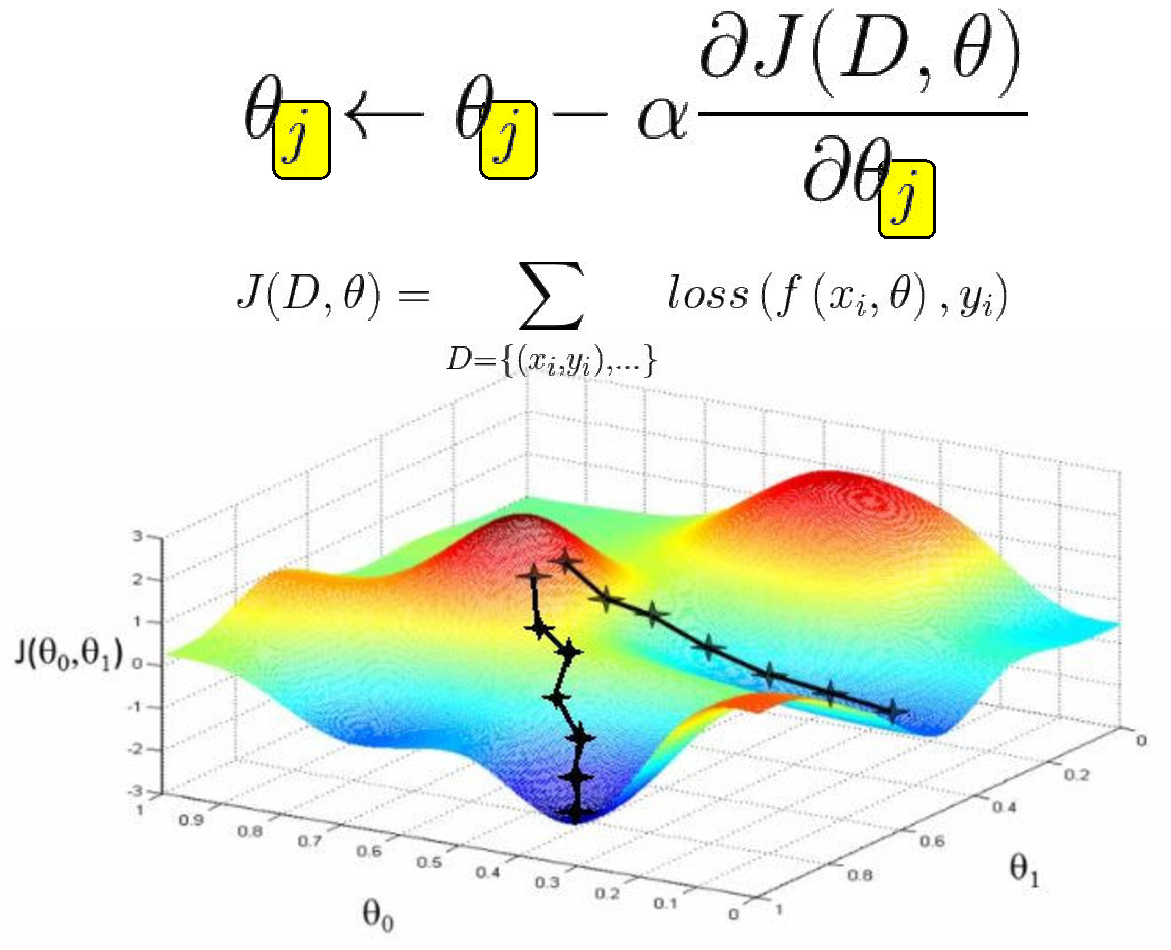
\includegraphics[width=0.8\linewidth]{gradient_descent.pdf}
    \caption{Gradientní sestup, $J$ značí objektivní funkci (chybu pro celý dataset), $D$ je dataset, $\theta$ jsou parametry.}
\end{figure}

%%%%%%%%%%%%%%%%%%%%%%%%%%%%%%%%%%%%%%%%%%%%%%%%%%%%%%%%%%%%%%%%%%%%%%%%%%%%%%%%

\section{Vyjádření neuronové sítě}

\begin{compactitem}
    \item Při práci s neuronovými sítěmi abstrahujeme od jednotlivým neuronů, vrstev, aktivačních funkcí, \dots

    \item Celá neuronová síť lze vyjádřit maticovým násobením a nebo grafem (orientovaný, acyklický).
\end{compactitem}

\subsection{Maticové násobení}

\begin{figure}[H]
    \centering
    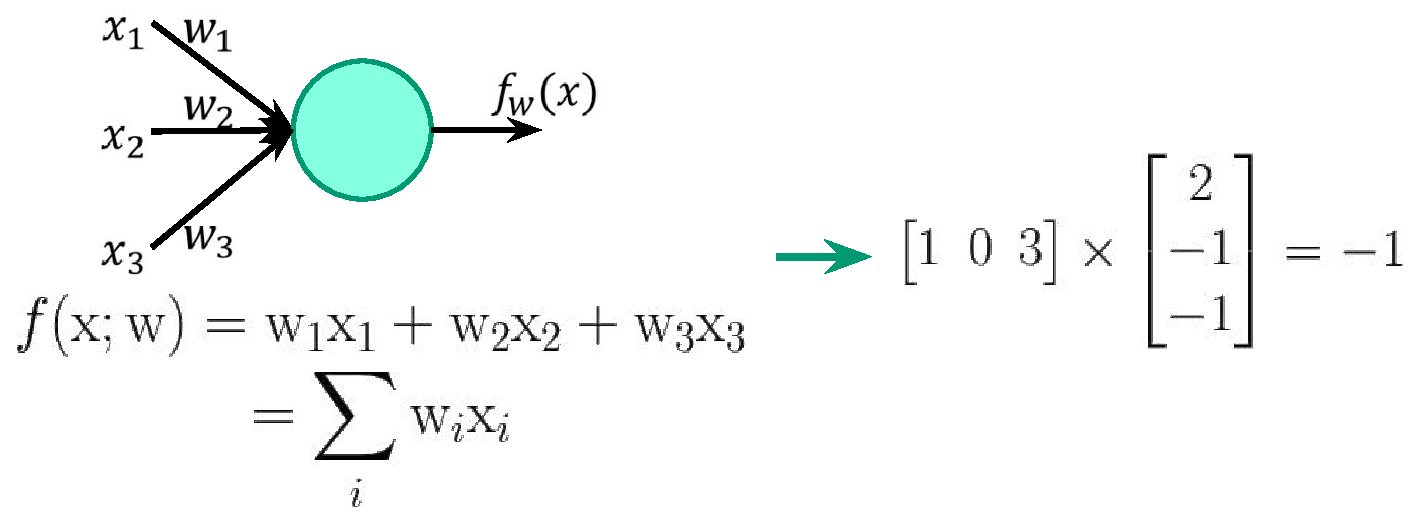
\includegraphics[width=0.65\linewidth]{nn_matrix_1.pdf}
    \caption{Vyjádření perceptronu pomocí násobení vektorů.}
\end{figure}

\begin{figure}[H]
    \centering
    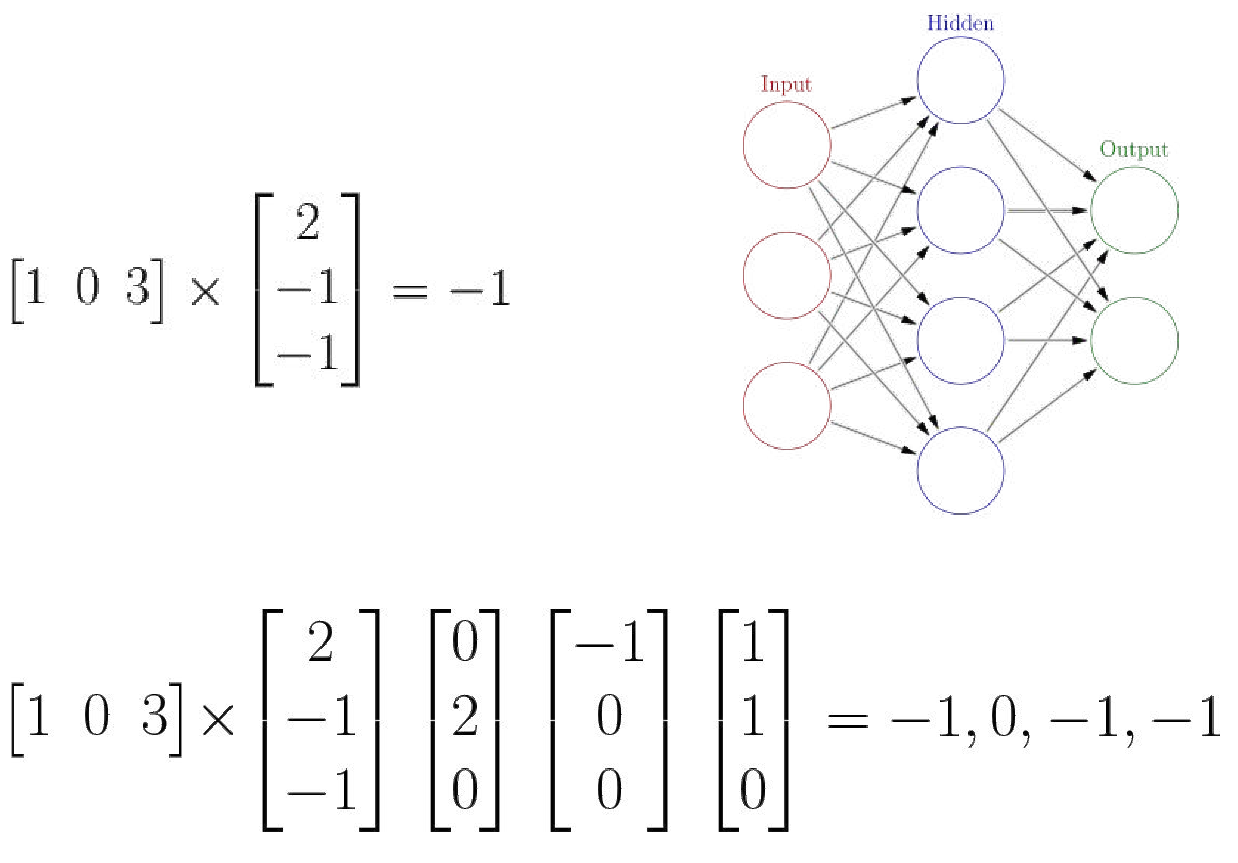
\includegraphics[width=0.65\linewidth]{nn_matrix_2.pdf}
    \caption{Vyjádření třívrstvé neuronové sítě pomocí násobení vektorů.}
\end{figure}

\begin{figure}[H]
    \centering
    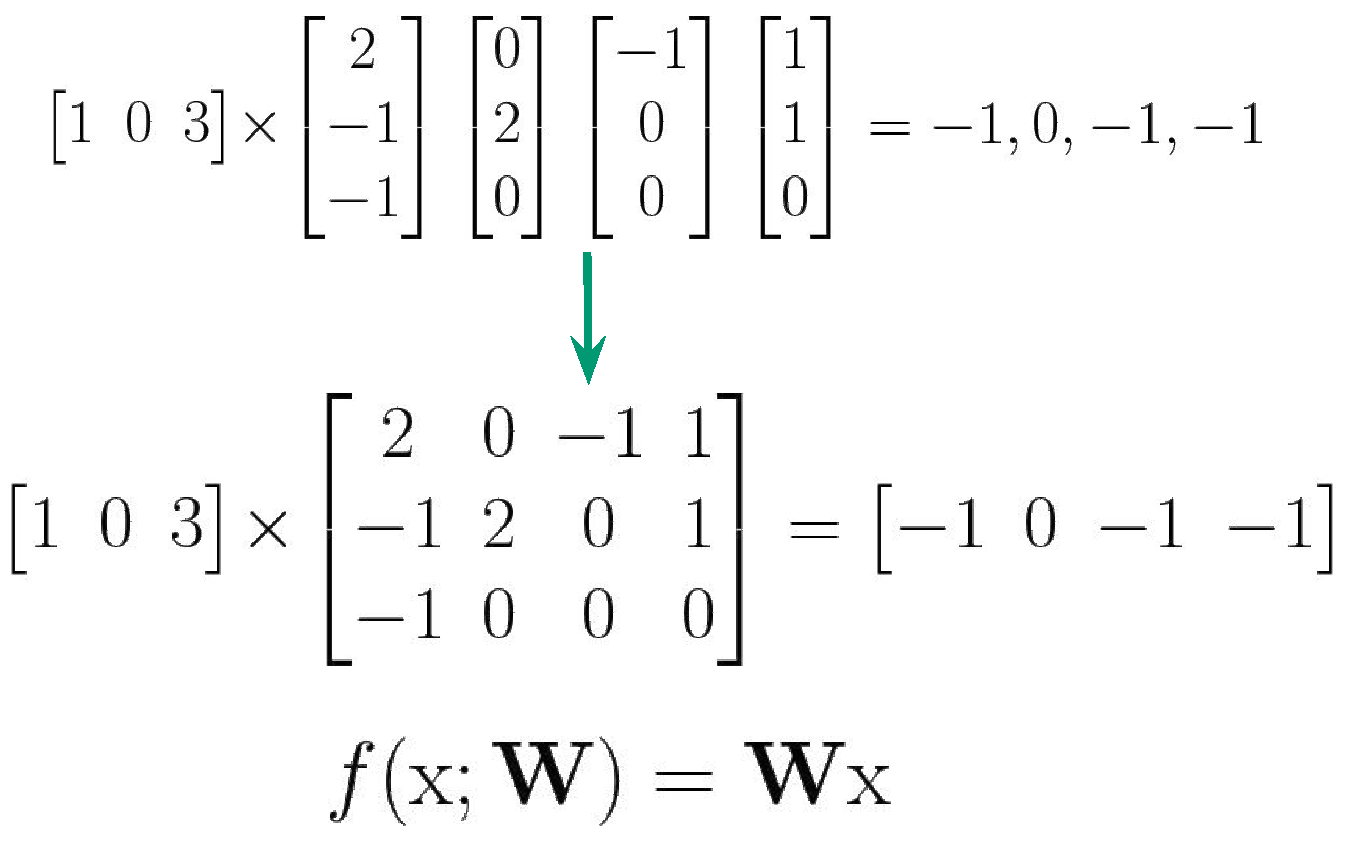
\includegraphics[width=0.65\linewidth]{nn_matrix_3.pdf}
    \caption{Vyjádření třívrstvé neuronové sítě pomocí násobení matic, $\mathbf{x}$ je vstupní vektor, $\mathbf{W}$ je vektor (matice) vah.}
\end{figure}

\subsection{Výpočetní graf}

\begin{figure}[H]
    \centering
    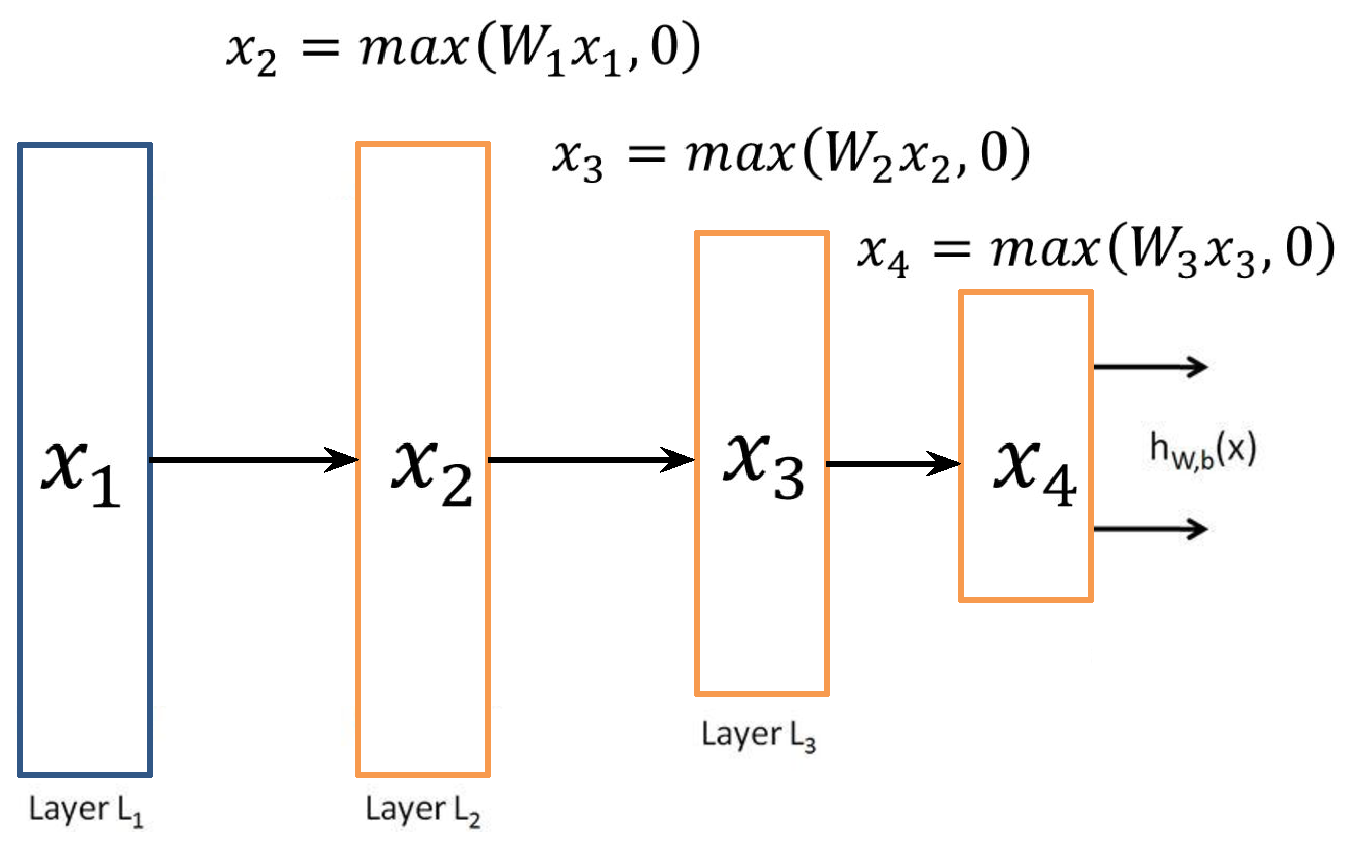
\includegraphics[width=0.65\linewidth]{nn_code.pdf}
    \caption{Vyjádření pomocí násobení matic lze transformovat velmi jednoduše do kódu, $x_i$ jsou mezivýsledky, $max$ je aktivační funkce, $W_j$ jsou váhy v jednotlivých vrstvách.}
\end{figure}

\begin{figure}[H]
    \centering
    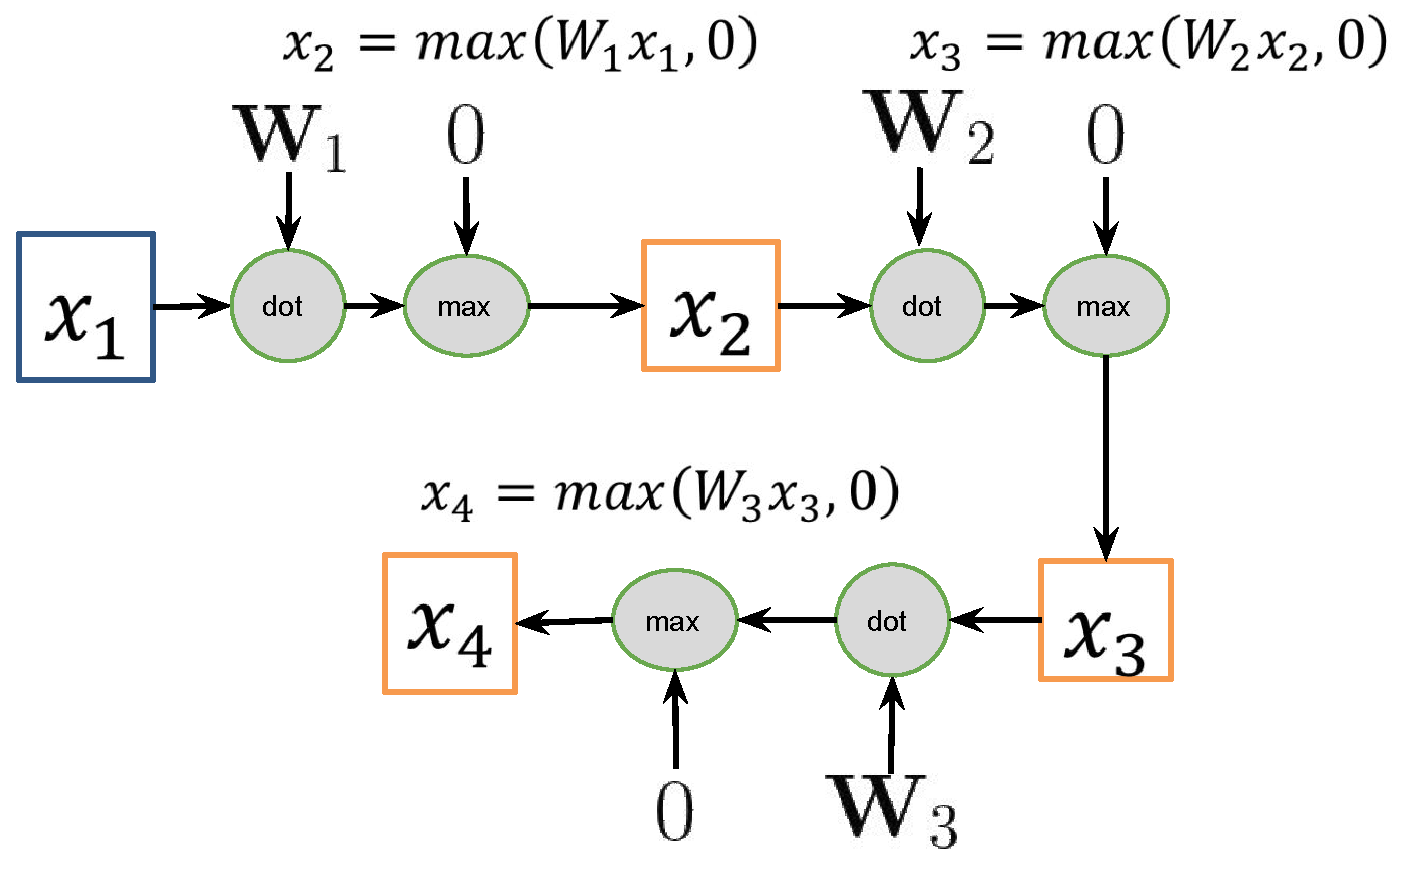
\includegraphics[width=0.7\linewidth]{nn_graph.pdf}
    \caption{Vyjádření v kódu, lze zapsat jako orientovaný, acyklický graf, $dot$ značí násobení.}
\end{figure}
